% E: x^2/4+y^2=1; Gamma: x^2+y^2=9. dmax=2<r=3.
\begin{center}
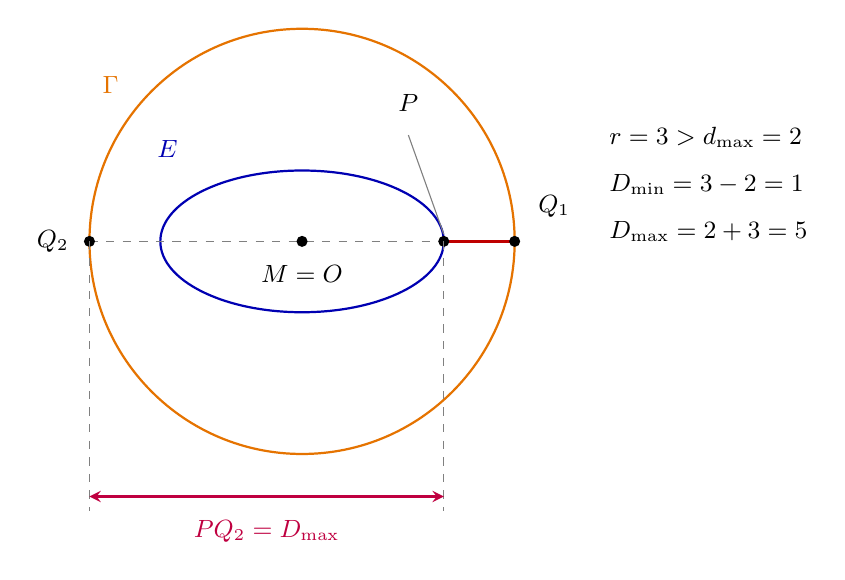
\begin{tikzpicture}[x=.9cm,y=.9cm,font=\small,>=stealth]
\draw[orange!90!black,thick] (0,0) circle(3);
\draw[blue!70!black,thick] (0,0) ellipse(2 and 1);
\draw[gray,dashed] (-3,0)--(3,0);
\draw[red!75!black,very thick] (2,0)--(3,0);
\fill (0,0) circle(2pt) node[below=5pt] {$M=O$};
\fill (2,0) circle(2pt);
\draw[gray] (2,.1)--(1.5,1.5) node[above=5pt,text=black] {$P$};
\fill (3,0) circle(2pt) node[above right=5pt] {$Q_1$};
\fill (-3,0) circle(2pt) node[left=4pt] {$Q_2$};
\node[blue!70!black] at (-1.9,1.3) {$E$};
\node[orange!90!black] at (-2.7,2.2) {$\Gamma$};
\node[anchor=west,align=left] at (4.2,.8)
 {$r=3>d_{\max}=2$\\[6pt]$D_{\min}=3-2=1$\\[6pt]$D_{\max}=2+3=5$};
\draw[gray,dashed] (-3,0)--(-3,-3.8) (2,0)--(2,-3.8);
\draw[<->,purple,thick] (-3,-3.6)--(2,-3.6) node[midway,below=5pt] {$PQ_2=D_{\max}$};
\end{tikzpicture}
\end{center}
